
\section{Description}

The program mainly utilized the concept of arrays to return a working 10-by-10
game board. To improve user experience, visual and audio elements were added to
the program interface. This feature is the significant purpose of using a
resource called \emph{SDL} or \href{https://www.libsdl.org/}{Simple DirectMedia Layer},
to render animation, play sound, and showcase creatives.

\begin{table}[H]
    \centering
    \def\arraystretch{2.5}
    \begin{tabular}{ c c c }
        \hline
        Instruction & Definition & Representation \\
        \hline
        O & Pacman & 
\includegraphics[scale=0.1]{assets/pacman_sample.png} \\
        $*$ & Food & 
\includegraphics[scale=0.1]{assets/food_sample.png} \\
        X & Blocks & 
\includegraphics[scale=0.1]{assets/block_sample.png} \\
        \$ & Door & 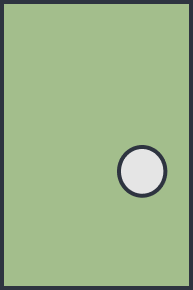
\includegraphics[scale=0.1]{assets/door_sample.png}\\
        \hline
    \end{tabular}
    \caption{The visual representation of symbols in the Ghostless Pacman game}
    \label{tab:1}
\end{table}

Pacman, instead of a a plain 'O' might definitely look more like Pacman. In fact, this Pacman actually munches. Rendering its animation is a feature of the said SDL
library. The same feature allowed the program to display food pieces as
something more delicious than asterisks or any other punctuation, that is,
cherries. The game obstacles that look tougher than 'X', and instead of a dollar
sign for the exit door, an exit door.\\

More than these, the resource is also used to render other images such as the overall interface of the game, including the menus, prompts, and warnings. Visual assets have been originally constructed using an online software called \href{https://www.figma.com/}{Figma}.\\

Another use of SDL is for the incorporation of sounds and music into the game. The audio assets used in the game are royalty-free and, if whose owner demands copyright, are given proper credit in About the Game.

In terms of functions, below are some that have been integrated into the program as the project requires:

\begin{enumerate}
    \item \codeword{fill_board_with_foods}\\
    \hspace{1em} This function will randomly fill the board with foods
    \item \codeword{fill_board_with_blocks}\\
    \hspace{1em} This function will randomly fill the board with blocks
    \item \codeword{check_if_player_won} and \codeword{check_player_status}\\
    \hspace{1em} These functions work hand-in-hand to check if the player reaches the exit sign after eating all the food pieces,
    or otherwise displays the player status of whether he or she wins or loses
\end{enumerate}